%************************************************
\chapter{Implementazione multiclasse}\label{ch:implementazione}
%************************************************

\section{Preparazione di uno stato quantistico}

Per analizzare dei dati classici attraverso un computer quantistico 
abbiamo bisogno di codificare in qualche modo le informazioni 
contenute nei nostri insiemi. Nel caso specifico, si parla delle 
coordinate dei vettori nello spazio delle caratteristiche e la 
classe associata ad ognuno di essi. 
Per fare questo, costruiamo degli stati quantistici 
ad hoc che rappresentino i vettori dati in maniera coerente. 
La procedura usata in questa tesi segue la tecnica di costruzione 
\ac{FF-QRAM} proposta da Park, Petruccione e Rhee \cite{petruccione}. 

\subsection{Flip-flop QRAM} \label{sec:ff-qram}

La \ac{FF-QRAM} è usata per memorizzare un \ac{QDB} inizializzato in maniera arbitraria. 
Nell'illustrare l'algoritmo di cotruzione verranno usati due registri quantistici: 
il primo, denotato genericamente $\ket{j}$, o con il pedice $B$, indica quale bus 
di memoria viene usato per il passaggio in corso, mentre il secondo, denotato 
$\ket{b_l}_R$, con il pedice $R$, sarà il registro che contiene i 
valori codificati del vettore dati. 
I vettori $\ket{j}_B$ vengono anche detti appartenere alla base computazionale. 
Lo stato finale dei qubit può essere 
arbitrario e l'ampiezza di probabilità $\psi_j$ con cui è accessibile ciascuno stato 
$\ket{j}_B$ della base computazionale codifica i valori classici di partenza. 

L'operazione QRAM sui qubit bus e registro sovrappone un insieme di dati classici 
$D = \left\{ \left( \vec{d}^{(l)}, b_l \right) | 0 \leq l < M \right\}$, dove 
$\vec{d}^{(l)}$ rappresenta $n$ bit di informazione e $b_l$ è il relativo attributo, come 
\begin{equation} \label{eq:qram}
    \text{QRAM}(D) \sum_j \psi_j \ket{j}_B \ket{0}_R \equiv 
    \sum_l \psi_l \ket{\vec{d}^{(l)}}_B \ket{b_l}_R,
\end{equation}

La \ac{FF-QRAM} è implementata sistematicamente con elementi comuni dei circuiti 
quantistici, che includono la porta di Pauli X controllata classicamente, $\overline{c}X$, 
e la porta di rotazione controllata da $n$ qubit, $C^n R_p (\theta)$. 
La $\overline{c}X$ inverte il qubit bersaglio solo quando il bit classico di 
controllo è zero. La porta $C^n R_p (\theta)$ ruota il qubit bersaglio di $\theta$ attorno 
all'asse $p$ della sfera di Bloch solo se tutti gli $n$ qubit sono 1. 

\begin{figure}[ht]
    \centering
    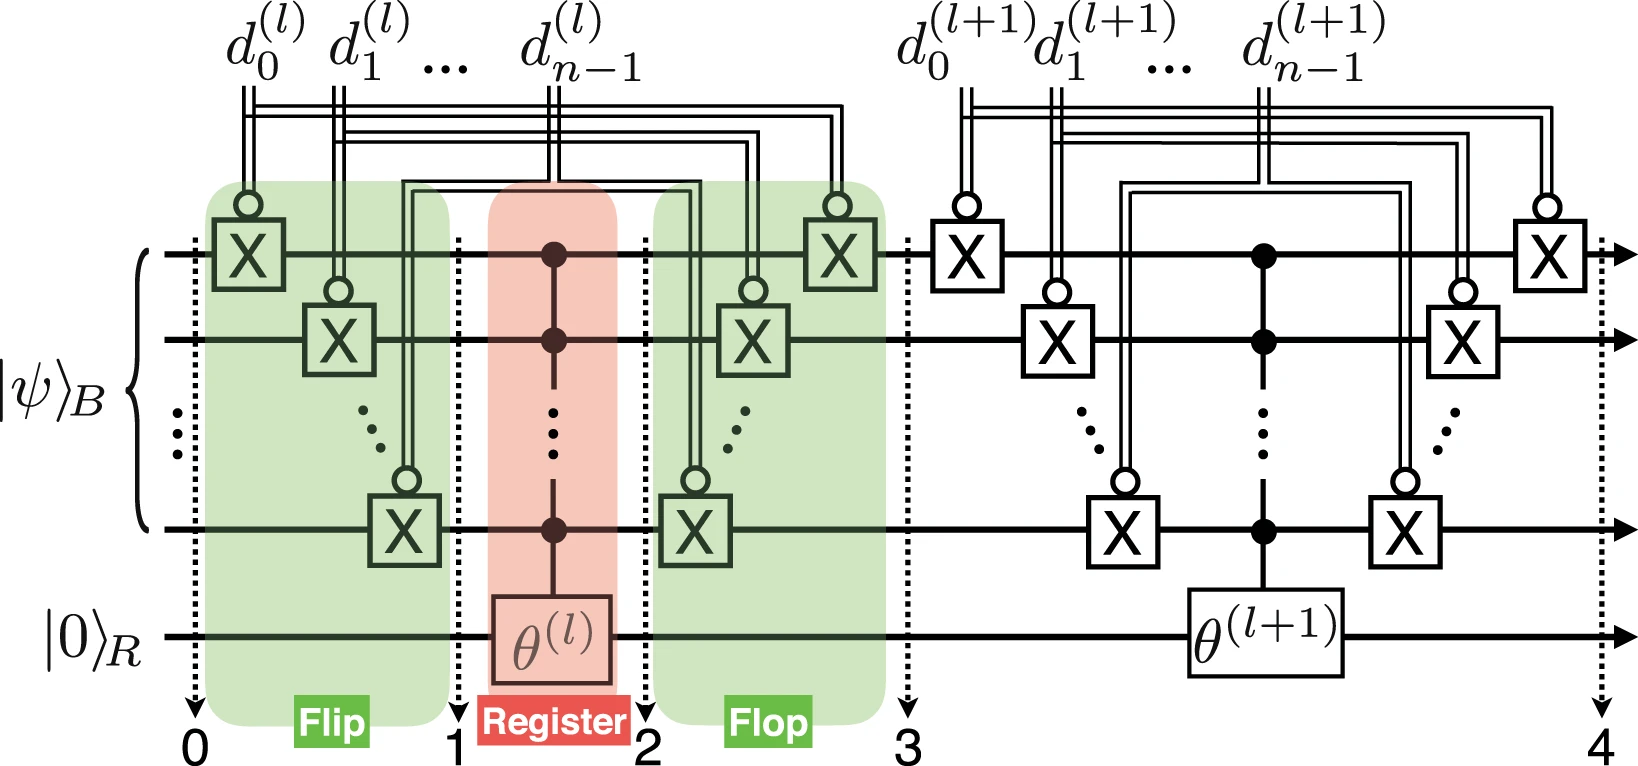
\includegraphics[width=\linewidth]{gfx/qram}
    \caption[Procedimento di costruzione FF-QRAM]%
    {Procedimento di costruzione FF-QRAM \cite{petruccione} \par \small 
    Circuito quantistico per \ac{FF-QRAM} che scrive
    le stringhe di bit $\vec{d}^{(l)}$ e $\vec{d}^{(l+1)}$ 
    come una sovrapposizione di stato quantistico con ampiezze 
    di probabilità determinate da $\theta^{(l)}$ e $\theta^{(l+1)}$ 
    rispettivamente, usando porte di rotazione controllate da più qubit. 
    Le linee doppie indicano operazioni controllate classicamente, 
    ed il cerchio vuoto (pieno) indica che la porta è attivata quando il 
    bit (qubit) di controllo è 0 (1). Le frecce tratteggiate e numerate 
    indicano i vari passaggi descritti nel testo principale.}
    \label{fig:qram}
\end{figure}

L'idea soggiacente al modello della \ac{FF-QRAM} è rappresentata in figura \ref{fig:qram}, 
che descrive la procedura per sovrapporre due stringhe di bit indipendenti 
$\vec{d}^{(l)}$ e $\vec{d}^{(l+1)}$ con ampiezze di probabilità desiderate 
nello stato del qubit bus $\ket{\psi}_B$. 
Lo stato iniziale può essere espresso focalizzandosi su $\vec{d}^{(l)}$ come 
\begin{equation}
    \ket{\psi_0}_l = \psi_{\vec{d}^{(l)}} \ket{\vec{d}^{(l)}} \ket{0}_R + \sum_{j \neq \vec{d}^{(l)}} 
    \psi_j \ket{j} \ket{0}_R,
\end{equation}
dove $\ket{\psi_s}_l$ denota lo stato degli ($n$) qubit nel processo di 
scrittura dell'$l$-esimo valore dati, osservato all'$s$-esimo passo in figura \ref{fig:qram}. 

Le porte $\overline{c}X$ controllate da $\vec{d}^{(l)}$ risistemano gli stati 
della base computazionale dei qubit bus cosicché $\ket{\vec{d}^{(l)}}$ diventa 
$\ket{1}^{\otimes n}$, ed il resto dei bit quantistici si invertono di conseguenza: 
\begin{equation}
    \ket{\psi_1}_l = \psi_{\vec{d}^{(l)}}\ket{1}^{\otimes n} \ket{0}_R + 
    \sum_{\ket{\overline{j \oplus \vec{d}^{(l)}}} \neq \ket{1}^{\otimes n} } \psi_j \ket{\overline{j \oplus \vec{d}^{(l)}}} 
    \ket{0}_R.
\end{equation}
La sovralinea nell'ultimo termine indica che l'inversione del bit avviene se il 
bit di controllo è 0. Dopo il passo 1, la rotazione controllata dai qubit, 
$C^n R_y(\theta^{(l)})$, denotata come $\theta^{(l)}$ nella figura, è applicata 
al qubit registro. Lo stato quantistico al passo 2 diventa 
\begin{equation}
    \ket{\psi_2}_l = \psi_{\vec{d}^{(l)}} \ket{1}^{\otimes n} \ket{\theta^{(l)}}_R + 
    \sum_{\ket{\overline{j \oplus \vec{d}^{(l)}}} \neq \ket{1}^{\otimes n} } \psi_j \ket{\overline{j \oplus \vec{d}^{(l)}}} 
    \ket{0}_R,
\end{equation}
dove $\ket{\theta}=\cos\theta\ket{0}+\sin\theta\ket{1}$. 
Le porte $\overline{c}X$ condizionate da $\vec{d}^{(l)}$ sono applicate di nuovo 
per far ritornare alla condizione precedente lo stato dei bus: 
\begin{equation}
    \ket{\psi_3}_l = \psi_{\vec{d}^{(l)}} \ket{\vec{d}^{(l)}} \ket{\theta^{(l)}}_R + 
    \sum_{j \neq \vec{d}^{(l)}} \psi_l \ket{j} \ket{0}_R.
\end{equation}

Il secondo giro registra i dati successivi di $\vec{d}^{(l+1)}$ e $\theta^{(l+1)}$: 
\begin{equation}
    \begin{split}
        &\ket{\psi_4}_{l,l+1} = \psi_{\vec{d}^{(l)}} \ket{\vec{d}^{(l)}} \ket{\theta^{(l)}}_R + \\
        &+ \psi_{\vec{d}^{(l+1)}} \ket{\vec{d}^{(l+1)}} \ket{\theta^{(l+1)}}_R + 
        \sum_{j \neq \vec{d}^{(l)},\vec{d}^{(l+1)}} \psi_j \ket{j} \ket{0}_R.
    \end{split}
\end{equation}
Questo processo può essere ripetuto tante volte quanti sono i dati da inserire. 
In questo modo, $M$ valori possono essere registrati con pesi non uniformi per 
generare lo stato 
\begin{equation}
    \sum_{l=0}^{M-1} \psi_{\vec{d}^{(l)}} \ket{\vec{d}^{(l)}} \left[ \cos\theta^{(l)} 
    \ket{0}_R + \sin\theta^{(l)} \ket{1}_R \right] + 
    \sum_{j \notin \{ \vec{d}^{(l)} \}} \psi_j \ket{j} \ket{0}_R.
\end{equation}
Infine, il \ac{QDB} richiesto nell'eq. \ref{eq:qram} può essere ottenuto 
selezionando un angolo $\theta^{(l)}$ appropriato che sia legato all'ampiezza di 
probabilità desiderata $b_l$, e postselezionando il risultato di misura $\ket{1}_R$. 
La probabilità di misurare $\ket{1}_R$ è 
\begin{equation} \label{eq:qram.prob}
    P(1) = \sum_{l=0}^{M-1} |\psi_{\vec{d}^{(l)}} \sin\theta^{(l)} |^2.
\end{equation}
Il costo per preparare uno stato con questo procedimento è di 
$\mathcal{O}(n)$ qubit e $\mathcal{O}(Mn)$ operazioni quantistiche. 

\section{Approccio multiclasse}

L'algoritmo \ac{QKNN} presentato in sezione \ref{sec:qknn} è stato implementato 
su un computer a 5 qubit, di cui solo 4 sono stati usati. La codifica usata prevedeva 
che un vettore bidimensionale $x = (x_0,x_1)$ normalizzato fosse codificato nello stato del 
qubit $\ket{i}$ come $\ket{\psi_x} = x_0 \ket{0} + x_1 \ket{1}$ attraverso una rotazione 
controllata dai qubit $\ket{a}$ e $\ket{m}$. Si faccia riferimento alla figura 
\ref{fig:circuito_schuld}. Parametrizzando l'angolo di Bloch attraverso la relazione 
\begin{equation}
    x_0 = \cos(\theta), \quad x_1 = \sin(\theta),
\end{equation}
otteniamo la relazione tra i vettori d'input e l'angolo $\theta$
\begin{equation}
    \theta = \arctan\frac{x_1}{x_0}. 
\end{equation}

\begin{figure}[h]
    \centering
    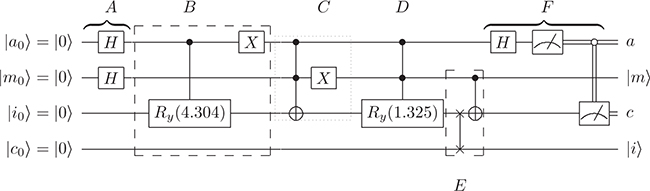
\includegraphics[width=\linewidth]{gfx/schuld_circuito}
    \caption{Il circuito quantistico base per il QKNN \cite{schuld}}
    \label{fig:circuito_schuld}
\end{figure}

La relazione appena mostrata è una delle prime che verranno modificate per permettere 
l'uso della \ac{QRAM}, quando si vorranno inserire vettori di dimensione maggiore di 2. 

Infatti, facendo riferimento all'eq. \ref{eq:qram.prob}, troviamo che lo stato costruito 
dopo la misura condizionale è 
\begin{equation}
    \sum_{l=0}^{M-1} \psi_{\vec{d}^{(l)}}\ket{\vec{d}^{(l)}}\sin\theta^{(l)}\ket{1}_R. 
\end{equation}
La relazione esistente tra i valori $b_l$, ovvero le componenti $x_i$, 
e le ampiezze di probabilità nella \ac{QRAM} è allora
\begin{equation} \label{eq:angolo.qram}
    \theta = \arcsin x_i. 
\end{equation}

L'espansione delle capacità del circuito prevede dunque l'aumento dei qubit 
dedicati a ciascun registro quantistico tra i seguenti: 
\begin{itemize}
    \item al registro $\ket{m}$ per aumentare i vettori di apprendimento; 
    \item al registro $\ket{i}$ per aumentare la dimensionalità dei vettori; 
    \item al registro $\ket{c}$ per aumentare il numero di classi riconosciute. 
\end{itemize}
Lo schema circuitale passa da quello mostrato in figura \ref{fig:circuito_schuld} a 
quello più generico mostrato in figura \ref{fig:qram_classi}. 

\begin{figure}[h!]
    \centering
    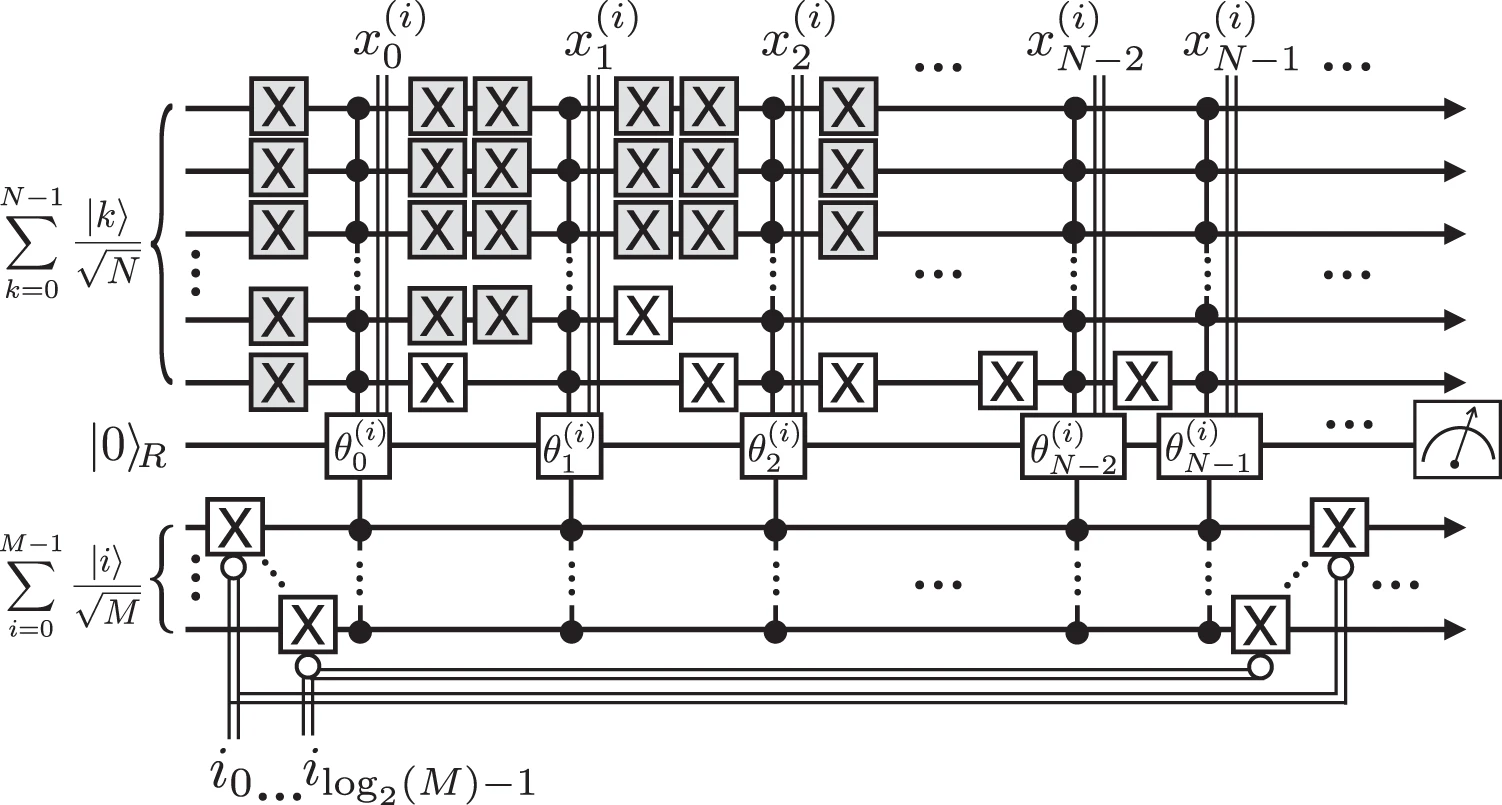
\includegraphics[width=\linewidth]{gfx/qram_classi}
    \caption[Circuito quantistico per preparare il \acs{QDB} per un quantum support vector machine]%
    {Circuito quantistico per preparare il \acs{QDB} per un quantum support vector machine \cite{petruccione} \par \small 
    Sono mostrate le porte per scrivere solo l'$i$-esimo vettore di apprendimento. Le porte ombreggiate 
    in grigio sono aggiunte esclusivamente per illustrare il processo flip-flop, e non sono implementate 
    in pratica.}
    \label{fig:qram_classi}
\end{figure}

La codifica del vettore d'input prevede che i qubit di controllo siano solo quelli mostrati 
nella parte superiore della figura. Al contrario, quando si codificano i vettori di 
apprendimento, li si pone in entanglement anche con i qubit indice $\ket{m}$ e 
classe $\ket{c}$, applicando le opportune porte $\overline{c}X$ all'inizio ed alla 
fine della loro codifica. 

Adottando una configurazione di esempio con 2 qubit indice, 2 qubit caratteristica e 
2 qubit classe si ottiene un classificatore capace di confrontare un vettore di 
input con 4 vettori di apprendimento aventi 4 caratteristiche ed appartenenti a 4 classi. 
Si riporta il codice relativo a tale realizzazione nel riquadro \ref{lst:multiclasse}. 

\begin{lstlisting}[float=h!,language=Python,frame=tb,caption={Algoritmo per il QKNN multiclasse},label=lst:multiclasse]
    a = QuantumRegister(1,'a') # knn ancilla
    m = QuantumRegister(2,'m') # training vector index
    i = QuantumRegister(2,'i') # feature index
    r = QuantumRegister(1,'r') # rotation qubit
    q = QuantumRegister(5,'q') # qram ancilla
    c = QuantumRegister(2,'c') # class
    b = ClassicalRegister(4, 'bit')
    circuit = QuantumCircuit(a,m,i,r,q,c,b)

    circuit.h(a)
    circuit.h(m)
    circuit.h(i)
    circuit.h(c)

    # circuit.cry(theta, control, target)
    # circuit.mcry(theta, controls, target, ancillae)

    # >>> Encode the input vector >>>

    encodeVector(circuit,inputVirginica,i,a[:]+i[:],r[0],q)

    circuit.x(a) # swap entanglement with ancilla to 0

    # <<< Encode the input vector <<<

    # >>> Encode the training vectors >>>

    buildTrainingState(trainingArray)

    # <<< Encode the training vectors <<<

    circuit.measure(r,b[0])

    circuit.h(a)

    circuit.measure(a,b[1])
    circuit.measure(c[0],b[2])
    circuit.measure(c[1],b[3])
\end{lstlisting}

La funzione \texttt{buildTrainingState} prende i vettori appartenenti a \texttt{trainingArray} 
e ne codifica i valori nelle ampiezze dei qubit attraverso la funzione mostrata 
nel riquadro \ref{lst:encodeTraining}. 

\begin{lstlisting}[float=h!,language=Python,frame=tb,caption={Funzione per codificare i vettori},label=lst:encodeTraining]
    def encodeTraining(circuit,data,i,controls,rotationQubit,ancillaQubits,c,m):
    # Header
    encodeClass(circuit,c)
    encodeIndex(circuit,m)
    
    # Encoder
    encodeVector(circuit,data,i,controls,rotationQubit,ancillaQubits)
    
    # Footer
    encodeClass(circuit,c)
    encodeIndex(circuit,m)
\end{lstlisting}

Le funzioni nell'header e nel footer altro non fanno che applicare le giuste porte X, 
come descritto in sezione \ref{sec:ff-qram} e in figura \ref{fig:qram_classi}. 
Più nello specifico, la funzione \texttt{encodeVector} applica le porte della parte 
superiore dell'immagine ed effettua le rotazioni controllate, 
mentre \texttt{encodeClass} e \texttt{encodeIndex} applicano 
quelle della parte inferiore\footnote{Per accedere al codice completo, fare riferimento 
alla cartella Script nella repository su GitHub \url{https://github.com/visika/Tesi}}. 

Nel capitolo successivo si discutono i risultati di classificazione ottenuti in 
caso di simulazione ed esecuzione su hardware quantistico. 

% Il quantum-enhanced machine learning (QEML) prova a rispondere alla domanda 
% se le proprietà quantomeccaniche come il parallelismo quantistico, 
% l'interferenza e i concetti di informazione quantistica possano essere usati 
% per migliorare gli algoritmi di machine learning classico. Il QEML è un campo 
% di ricerca relativamente nuovo, dimostrato dal fatto che il termine 
% \emph{quantum machine learning} è stato coniato solo nel 2013 in un manoscritto 
% di Lloyd, Mohseni e Rebentrost (2013). % inserire fonte *******************
% Dal 1995 in poi, molti algoritmi di QEML sono stati pubblicati, come riassunto 
% nel recente articolo di revisione di Biamonte et al. (2016). % inserire fonte **
% Per ottenere accelerazioni quantistiche, molti algoritmi di QEML usano procedure
% quantistiche ben note, come l'algoritmo di ricerca di Grover, la trasformata di 
% Fourier quantistica o la quantum phase estimation come sottoprocessi per compiti
% di machine learning più grandi. % inserire fonti **********************

% Il machine learning classico prende dati classici in entrata ed impara da essi 
% usando algoritmi classici eseguiti su computer classici: Aïmeur % aggiungi fonti
% si riferiscono a questo come C/C (dati classici con algoritmi classici). 
% Si entra nel campo del \ac{MLQ} generico quando uno tra dati quantistici e 
% algoritmi quantistici è combinato con il machine learning. Ebbene, Aïmeur 
% % aggiungi fonti *************************************
% dividono il campo del machine learning quantistico in tre diversi sottocampi: 
% \begin{itemize}
%     \item C/Q: dati classici con algoritmi quantistici;
%     \item Q/C: dati quantistici con algoritmi classici;
%     \item Q/Q: dati quantistici con algoritmi quantistici.
% \end{itemize}
% Così, i dati quantistici includono qualsiasi dato descrivente un sistema 
% quantomeccanico come p.e. l'hamiltoniana o il vettore d'onda di un sistema 
% quantistico.

% Il sottocampo Q/C elabora dati quantistici con algoritmi di machine learning 
% classico. Per esempio, Carrasquilla e Melko (2016) % aggiungi fonti *******
% hanno usato il pacchetto di deep learning TensorFlow di Google per identificare 
% transizioni di fase in sistemi quantistici. Il sottocampo Q/Q è l'unione di 
% C/Q e Q/C e ha a che fare con l'elaborazione di dati quantistici attraverso 
% l'uso di algoritmi quantistici p.e. imparare come è fatta l'hamiltoniana di un 
% sistema quantistico unsando algoritmi di machine learning quantistico. Questo 
% lavoro di tesi è immerso nel sottocampo C/Q, anche chiamato QEML, che mira a 
% sviluppare algoritmi quantistici per compiti di machine learning che coinvolgono 
% dati classici. 

% Le sezioni seguenti introdurranno alcuni dei concetti fondamentali dal campo 
% del QEML. Più nello specifico, la sezione 4.2 % rivedere ********************
% presenta la versione quantistica dell'algoritmo k-nn classico, la cui simulazione
% ed esecuzione quantistica saranno discussi nel capitolo 5. 
% % Quindi il capitlo 5 discuterà i risultati
% In ogni caso, dato che un algoritmo quantistico è una sequenza di porte 
% quantistiche, può solo manipolare bit quantistici e non classici. 
% Dunque, la prossima sezione descriverà prima come dei dati classici possano 
% essere trasferiti in degli stati quantistici, in modo da permettere 
% l'elaborazione quantistica. 

% La preparazione di uno stato quantistico è il procedimento in cui si prepara 
% uno stato quantistico che rappresenta accuratamente un vettore contenente 
% dati classici (normalizzati). Per applicare qualsiasi algoritmo di machine 
% learning quantistico a dati classici, la preparazione dello stato quantistico 
% deve sempre essere eseguita prima. Perciò, bisogna diventare familiari 
% con le nozioni di preparazione degli stati quantistici prima di procedere nelle 
% sezioni avanzate di questa tesi. Ci sono due modi fondamentalmente diversi 
% di codificare dei dati classici in stati quantistici ma in questa tesi ne verrà 
% usato solo uno. Il primo modo consiste nel codificare lo stato dei bit classici 
% che appartengono ai nostri dati direttamente negli stati dei singoli qubit: 
% al bit 0 viene fatto corrispondere un qubit nello stato $\ket{0}$ ed al bit 1 
% un qubit nello stato $\ket{1}$. Una ricetta per effettuare una tale operazione 
% è descritta da Trugenberger (2001). % inserisci fonte ******************
% Una maniera più raffinata di rappresentare un vettore classico come uno stato 
% quantistico, che è quella che verrà adottata, sfrutta le $2^n$ ampiezze di un 
% sistema di $n$ qubit. In questo modo un vettore $k$-dimensionale può essere 
% codificato usando solo $\log_2(k)$ qubit, poiché abbiamo visto che il numero 
% di ampiezze disponibili cresce esponenzialmente con il numero dei qubit. 
% Questo tipo di memorizzazione dei dati apre le porte ad una compressione 
% esponenziale dei dati classici. 

% Se si ha un vettore classico e lo si vuole codificare nelle ampiezze si può fare 
% la seguente operazione 
% \begin{equation}
%     \begin{pmatrix}
%         0.6\\0.4
%     \end{pmatrix}
%     \arrowvert
%     \ket{n} = \sqrt{0.6}\ket{0} + \sqrt{0.4}\ket{1}.
% \end{equation}

% Se abbiamo un insieme di M dati classici rappresentati come 
% % $D = \{ (\vec{d}^{(l)}), b_l \} | 0 \leq l < M}$, dove $\vec{d}^{(l)}$ rappresenta 
% n bit di informazione, ovvero l'indirizzo del registro, a cui è associato il dato 
% $b_l$ (che può essere un valore binario o reale), possiamo costruire uno stato 
% quantistico che soddisfi la seguente relazione: 
% \begin{equation} \label{eq:qdb}
%     % \ket{\psi}_{QDB} = \sum_{l=0}^{M-1}b_l\ket{\vec{d}^{(l)}}
% \end{equation}
% QDB è quantum database. 
% Stiamo dicendo che conserviamo ogni valore $b_l$ in una ampiezza dei qubit a disposizione. 

% commento sulla postselezione **********************

% continua a inserire dall'articolo ***********************************

% I dettagli tecnici verranno descritti nella appendice. 

% si potrebbe dire che cos'è una QRAM
